\subsection{Cenni teorici}
Un \textit{Algoritmo Genetico} GA è una tecnica metaeuristica per risolvere problemi di ricerca e ottimizzazione che riproduce il processo evolutivo della specie umana.

Si considera una popolazione di individui che rappresentano delle possibili soluzioni per un certo problema. La qualità di un individuo (cioè quanto è buona la soluzione per il problema) è misurata mediante una funzione di \emph{fitness}. In un certo senso, la funzione di \emph{fitness} indica l’adattabilità all’ambiente: gli individui che meglio si adattano ("fit") hanno piú probabilità di riprodursi e di trasmettere i propri geni alle generazioni future. Un GA risulta quindi una procedura di ricerca iterativa il cui scopo è l’ottimizzazione della funzione di \emph{fitness}. Partendo da una popolazione iniziale, un GA produce nuove generazioni che contengono (di solito) individui migliori delle precedenti, evolvendo verso una soluzione ottimale (locale o globale) del problema assegnato. Infatti non è garantito che un GA trovi una soluzione globalmente ottima ma è in grado di trovare soluzioni buone in tempi ragionevoli.

Ogni individuo della popolazione rappresenta un punto nello spazio di ricerca e i più importanti operatori di ricerca sono la \emph{ricombinazione} (o \emph{crossover}) e la mutazione. Il \emph{crossover} combina i geni tipicamente di due individui per produrre individui figli che ereditano caratteristiche da entrambi i genitori. La \emph{mutazione} reintroduce nella popolazione materiale genetico perduto.

La ricerca genetica realizza un compromesso tra "exploitation" della miglior soluzione disponibile ed "exploration" dello spazio delle soluzioni. Exploitation ed exploration corrispondono, rispettivamente, a ricerca locale e ricerca globale: "exploitation" eccessiva può portare l’algoritmo a convergere ad una soluzione non accettabile (la ricerca resta intrappolata in un ottimo locale), "exploration" eccessiva può non sfruttare appropriatamente la conoscenza già disponibile rendendo il processo di ricerca molto lento (un esempio è la ricerca casuale).

\subsection{Codifica della soluzione}
La nostra implementazione di algoritmo genetico prende spunto dai paper \cite{Jakobs} e \cite{Hopper} adattandoli al nostro problema, dato che trattano la variante su singolo bin.

Per prima cosa si è scelto come codificare una soluzione del problema (fenotipo) nella sua rappresentazione nello spazio di ricerca (genotipo). Nel nostro caso una soluzione del problema o fenotipo consiste nel layout dei pacchetti (o packing pattern) nei vari bin e dunque la sua rappresentazione naturale è basata sulle coordinate di ciascun pacchetto all'interno dei bin corrispondente. Usare questa rappresentazione nello spazio di ricerca risulterebbe però complicato dato che piccole modifiche alle coordinate porterebbero probabilmente alla sovrapposizione dei pacchetti e dunque a una soluzione non ammissibile. Si è dunque deciso di assegnare un indice a ciascun pacchetto e rappresentare il layout attraverso una loro permutazione, indicante l'ordine in cui sono stati inseriti secondo l'algoritmo BLF.
\begin{figure}[htb]
  \centering
  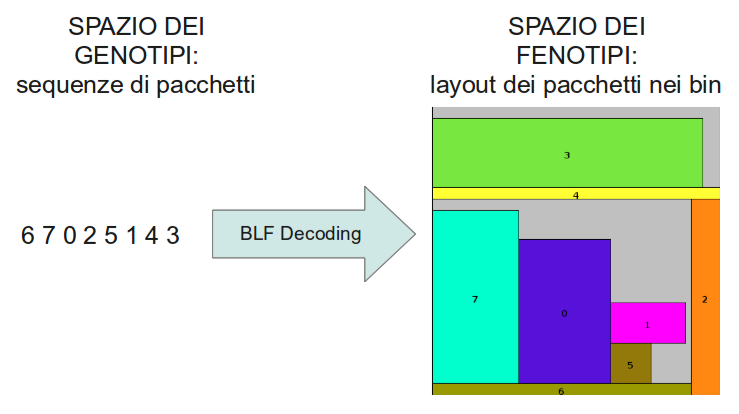
\includegraphics[height=0.4\textwidth]{./img/encoding.png}
  \caption{Esempio di decodifica di una sequenza di packing}
  \label{img:encoding}
\end{figure}
\subsection{Funzione di fitness}
Il passo sucessivo è stato decidere come valutare la \emph{fitness} di ciascun individuo. Trattandosi di un problema di minimizzazione abbiamo deciso di assegnare a individui migliori valori di \emph{fitness} inferiori. In questo modo il valore della funzione di \emph{fitness} può esprimere a colpo d'occhio quanti sono i bin impiegati:

\[
   fitness(layout)= 100\cdot nBins + 49(\alpha\frac{H}{binsHeight}+\beta\frac{A}{binsArea})
\]

Si osservi infatti come la fitness sia costituita da una componente dipendente dal numero di bin occupati e da una penalità che a parità di bin permette di discriminare quale sia la soluzione migliore. In particolare questa penalità è una funzione dell'altezza \emph{$H$} e dell'area occupata \emph{$A$} nel bin con minor area occupata. Questi 2 valori sono poi normalizzati rispetto ad altezza ed area dei bin e moltiplicati per i coefficienti \emph{$\alpha$} e \emph{$\beta$} che rappresentano i pesi che si vogliono assegnare rispettivamente ad altezza e densità. Infine un fattore di scala permette di far spaziare maggiormente questa penalità mantenendola sempre al di sotto del centinaio.
Va notato inoltre che la \emph{fitness} è associata al layout e non direttamente alla sequenza di packing. Questo implica che ogniqualvolta la sequenza viene modificata è necessario ricalcolare il layout ad essa associato invocando la routine di BLF.
\subsection{Algoritmo}
Ecco lo pseudocodice dell'algoritmo:
\texttt{\footnotesize
   \begin{tabbing}
   \=~~~\=~~~\=~~~\=~~~\\
   Algoritmo Genetico(...)\\\\
   inizializza casualmente una $popolazione$ di individui\\
   while (not(condizione di stop)) do\\
   \>\>seleziona individui dalla popolazione e mettili nel $matingPool$\\
   \>\>applica crossover ad individui del $matingPool$ e mettili nell'$offspringPool$\\
   \>\>applica mutazioni all'$offspringPool$\\
   \>\>rimpiazza i peggiori della $popolazione$ con i migliori offspring\\
   end while\\\\
   end\\
   \end{tabbing}
}
Per prima cosa viene inizializzata casualmente la popolazione, definendo il genotipo di ciascun individuo come una permutazione casuale della sequenza di packing, e valutandone il layout e la relativa \emph{fitness}.
Successivamente l'algoritmo entra in un ciclo in cui ogni iterazione corrisponde ad una generazione della popolazione. Le condizioni di terminazione dell'algoritmo sono:
\begin{itemize}
\item sono state generate \emph{n} iterazioni, con \emph{n} fissato;
\item tutti gli individui della popolazione possidono lo stesso corredo genetico ossia stessa sequenza di packing;
\end{itemize}
Inoltre, al termine di ogni iterazione, si tiene traccia del miglior individuo visto fino a quel momento. Quando una delle condizioni di terminazione verrà raggiunta tale individuo rappresenterà la soluzione finale del problema.
Vediamo ora nel dettaglio che cosa succede esattamente ad ogni iterazione.
\begin{figure}[htb]
  \centering
  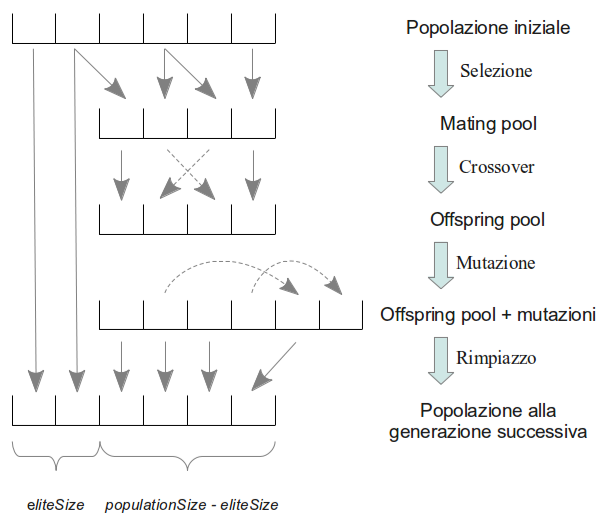
\includegraphics[height=0.4\textwidth]{./img/geneticIteration.png}
  \caption{Schema di funzionamento di una singola iterazione}
  \label{img:geneticIteration}
\end{figure}
\subsection{Selezione}
La selezione ha un duplice scopo:
\begin{itemize}
\item favorire la riproduzione di individui con \emph{fitness} bassa;
\item preservare la diversità della popolazione in modo da esplorare tutte le regioni dello spazio di ricerca;
\end{itemize}
Si è deciso di implementare una \emph{Tournament Selection} in accordo con quanto descritto in \cite{TournamentSelection}. In pratica si definisce un parametro \emph{tournamentSize} che indica appunto il numero di partecipanti a ciascun torneo, che verranno scelti a caso dalla popolazione. In ogni torneo il vincitore è l'individuo con \emph{fitness} minore e viene messo nel \emph{mating pool}.

Si è scelto di usare la \emph{Tournament Selection} in quanto è un meccanismo robusto, semplice da implementare, e permette di regolare attraverso il parametro \emph{tournamentSize} la \emph{selection pressure} ossia il grado con cui i migliori individui sono favoriti: più è grande la dimensione del torneo e più sono favoriti nella selezione gli individui migliori.

\subsection{Crossover}
Lo scopo principale del \emph{crossover} o \emph{riproduzione} è quello di trasmettere porzioni "buone" delle sequenze di packing dei genitori ai figli e quindi alle generazioni successive. Per far questo abbiamo sviluppato una tipologia di \emph{crossover} che a partire da 2 genitori crea 2 figli nel seguente modo:
\begin{itemize}
\item date le sequenze di packing dei genitori, sceglie a caso un punto di spezzamento \emph{p} all'interno di tali sequenze e un certo numero \emph{q} di geni da copiare nei figli;
\item viene copiata la porzione di sequenza delimitata dagli indici [\emph{p, p+q-1}]: dal padre in un punto casuale del primo figlio, e dalla madre in un punto casuale del secondo figlio;
\item la sequenza del primo \emph{offspring} viene poi completata con gli indici dei pacchetti mancanti (inserendoli prima e dopo la porzione copiata), nell'ordine in cui si incontrano nel genotipo della madre. Allo stesso modo il secondo \emph{offspring} viene completato nell'ordine in cui si incontrano nel padre;
\item infine i due offspring vengono inseriti nell'\emph{offspring pool} sul quale verranno poi eventualmente eseguite le mutazioni;
\end{itemize}

\begin{figure}[htb]
  \centering
  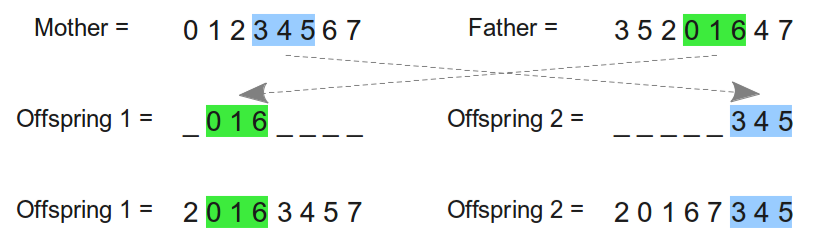
\includegraphics[height=0.25\textwidth]{./img/crossover.png}
  \caption{Esempio di crossover con p=3  e q=3}
  \label{img:crossover}
\end{figure}

Questa tipologia di crossover costituisce una piccola rivisitazione del PMX usato da Goldberg nel problema del TSP ed è in grado di essere eseguita in tempo lineare nel numero di pacchetti della sequenza. Inoltre abbiamo poi definito un parametro \emph{pCrossover} che definisce la probabilità con cui una coppia di individui esegue questa ricombinazione. In caso questa non avvenga, i genitori vengono inseriti senza modifiche nell'\emph{offspring pool}.

\subsection{Mutazioni}
Abbiamo previsto 3 tipologie di mutazioni per la sequenza di packing di un individuo:
\begin{itemize}
\item \emph{rotation based}: definisce la probabilità \emph{pRotation} con cui ogni singolo packet all'interno della sequenza viene ruotato;
\item \emph{swap based}: per ogni packet di una sequenza di un individuo con probabilità \emph{pSwap} questo viene scambiato con un'altro a caso nella sequenza;
\item \emph{order based}: ogni packet di una sequenza di un individuo con probabilità \emph{pOrder} viene spostato in una posizione casuale della sequenza shiftando a destra la parte rimanente della sequenza;
\end{itemize}
